\documentclass[a4paper, 11pt]{article}
\usepackage[magyar]{babel}
\usepackage{t1enc}
\usepackage{graphicx}
\usepackage{hyperref}
\usepackage{placeins}


\begin{document}

\begin{titlepage}

    \begin{center}
        \vspace{0.3cm}
        \textbf{Budapesti Műszaki és Gazdaságtudományi Egyetem}\\
        \textmd{Intelligens elosztott rendszerek (BMEVIMIAC02)}\\[5cm]

        {\huge \bfseries Házi feladat }\\[0.8cm]
        {\huge \bfseries Okos kereszteződés }\\[0.8cm]
        \vspace{5.5cm}
        \Large \textbf{Pap Arion}(YJWQMP)\\
        \Large \textbf{Rippl Balázs Róbert}(FLHM6J)\\

        \vspace{1cm}
        \textsc{\Large \today}\\

    \end{center}
\end{titlepage}
\tableofcontents
\newpage

\section{A választott feladat leírása}
Házifeladatunkként egy intelligens kereszteződést valósítottunk meg.
A kereszteződésben kizárólag gépkocsi forgalom megengedett, tehát zebrák nincsenek.
4 irányból érkezhetnek az autók, aszinkron módon, ezek mindegyike egy ágens,
amelyek kommunikálnak egymással. Amint kilép egy ilyen ágens a képernyőről, egy másik,
véletlenszerű pozícióban újra megjelenik. Az autók ezen felül tudnak sávot váltani,
amennyiben szükséges ez a célpozíciójuk eléréséhez. Az autók kék színnel vannak megjelenítve.

A kereszteződés feladata, hogy optimális sorrendben váltsa zöldre a lámpákat, minimalizálva
az autók által a pirosnál eltöltött időt. A lámpák két másodpercig zöldek, majd két másodperces
teljes tiltási időszak következik, hogy a kereszteződés kiürülhessen.

Mind a 4 irányba 2x3 sávos utak vezetnek, amelyek közül
a bal oldaliból csak balra, a középsőből csak egyenesen, a jobb oldaliból csak jobbra folytathatják
az útjukat a gépkocsik.

Manuálisan be tudunk avatkozni a program működésébe,
hiszen 4 darab nyomógomb megjelenik a felhasználói ablak alján TOP, RIGHT, BOTTOM, LEFT feliratokkal,
amelyek azt az irányt jelölik, ahonnan érkezni fog a gomb hatására egy mentőautó.
Ez a modellünk kritikus eseménye, ekkor az a lámpa, amely ahhoz a sávhoz tartozik,
amelyben a mentőautó tartózkodik, automatikusan zöldre vált, ezzel utat biztosítva a mentőautónak.
A mentőautó alapszíne narancssárgás.

\section{A megoldás összefoglalása}
\subsection{Ágensek}
\subsubsection{Személyautó ágens}
Az autó ágensek célja a véletlenszerű születési pontból biztonságosan és szabályosan eljutni a céloldalra.
Indulás után elkezdenek haladni a kereszteződés felé, miközben folyamatosan figyelik, át tudnak-e sorolni
a megfelelő sávba. Ez élvez prioritást, tehát ha egy autó ágens a balra kanyarodó sávban tartózkodik, de
az ő célja a szembe oldal, tehát a középső, egyenesen tartó sávban kell belépjen a kereszteződésbe, akkor
ha van lehetősége inkább sávot fog váltani, mint előre haladni.

Az autó ágensek feltétlen célja az ütközés elkerülése. Amennyiben nem kell sávot váltani, vagy éppen nem
lehet mert van egy másik autó ágens az adott sávban, illetve az ágens előtt is, vagy a piros lámpa, az ágens
tehetetlenül megáll, és addig vár, amíg nem szabadul fel valamelyik helyzet.

Miután az autó ágens sikeresen
bejut a kereszteződésbe, már nincs értelme tovább gondolkodnia, a ráfutást elkerülve ugyan, de már csak 
elhagyja a kereszteződést. Ha az ágens elérte végső célját, a modellezett terület szélét a megfelelő oldalon,
megsemmisítésre kerül, és helyébe új születik.

Az autók darabszáma fordítási időben módosítható paraméter.
	
\subsubsection{Lámpa ágens}
A lámpa ágensek megfelelő jelzések esetén pirosra, illetve zöldre váltanak, ezzel átengedve vagy megállítva az érkező járműveket.
Feladatuk még a sávjukban felgyűlt autók értékeinek aggregálása, majd a kapott érték meglicitálása a 
hirdetett aukciókon. Egyfajta híd szerepet töltenek be a központ és az autók között.

Lámpa ágensből minden sávhoz tartozik egy, tehát fixen 9 darab található meg a szervezetben.
\subsubsection{Vezérlő ágens}
A vezérlő ágens feladata a kereszteződés irányitási ciklusának meghatározása. Megadott időközönként
tiltó jelet küld minden lámpának, ezzel felkészítve a kereszteződést egy újabb zöldhullámra.
Mikor lejár a türelmi időszak, aukciót hirdet a lámpák között. Az aukció nyertese feltétlenül jogosult
lesz zöldre váltani.

A központtól azonban elvárt, hogy ennél hatékonyabban irányítsa a forgalmat.
Az aukción részt vevő lámpákat a licitjükben nézve sorban engedélyezi, ha az adott lámpának a forgalma
nem keresztezi egyik, már engedélyezett lámpának a forgalmát sem.
\subsubsection{Mentőautó ágens}
A modellezett környezet kritikus eseménye egy megkülönböztetett jármű, a mentőautó megjelenése.
Az ágens sokmindenben megegyezik az autó ágenssel: ugyanaz a célja és nagyon hasonló a mozgása, bár jóval
gyorsabb.

A különbség a lámpához való bejelentkezésben rejlik. A mentőautó esetében nem foglalkozunk azzal,
hogy mióta áll a pirosnál, hanem sokkal nagyobb értékben vesszük figyelembe, ezzel szinte garantálva, hogy mielőbb
átjuthasson a kereszteződésen.

Mentőautó ágensből kizárólag egy szerepelhet egyidőben a modellben.

\subsection{Ágensek közötti kapcsolatok}
A járművek helymeghatározó rendszerrel vannak ellátva, amik sugározzák a jármű adott pozícióját. Így
a járművek helyzetét minden ágens érzékelni tudja a környzetből.

A járművek direkt kommunikációt alkalmaznak az értékük (autók esetében várakozási idejük, mentőautó
esetén egy fix, magas érték) közlésére. Konkrétan a sávjukhoz tartozó lámpának címezve üzenik meg azt,
amit a lámpák fogadnak és feltétlenül elhisznek.

A lámpák és a központ között többféle kommunikáció is megvalósul.

A központ broadcast üzenetben közli a lámpákkal, amikor pirosra kell váltani, majd direkt 
kommunikációt alkalmazva értesíti azokat, akik zöldre válthatnak.

Az aukció meghirdetése egy kérdés formájában zajlik. A lámpa ágensek erre a kérdésre válaszolva
teszik meg licitjeiket az aukción.

\begin{figure}
    \centering
    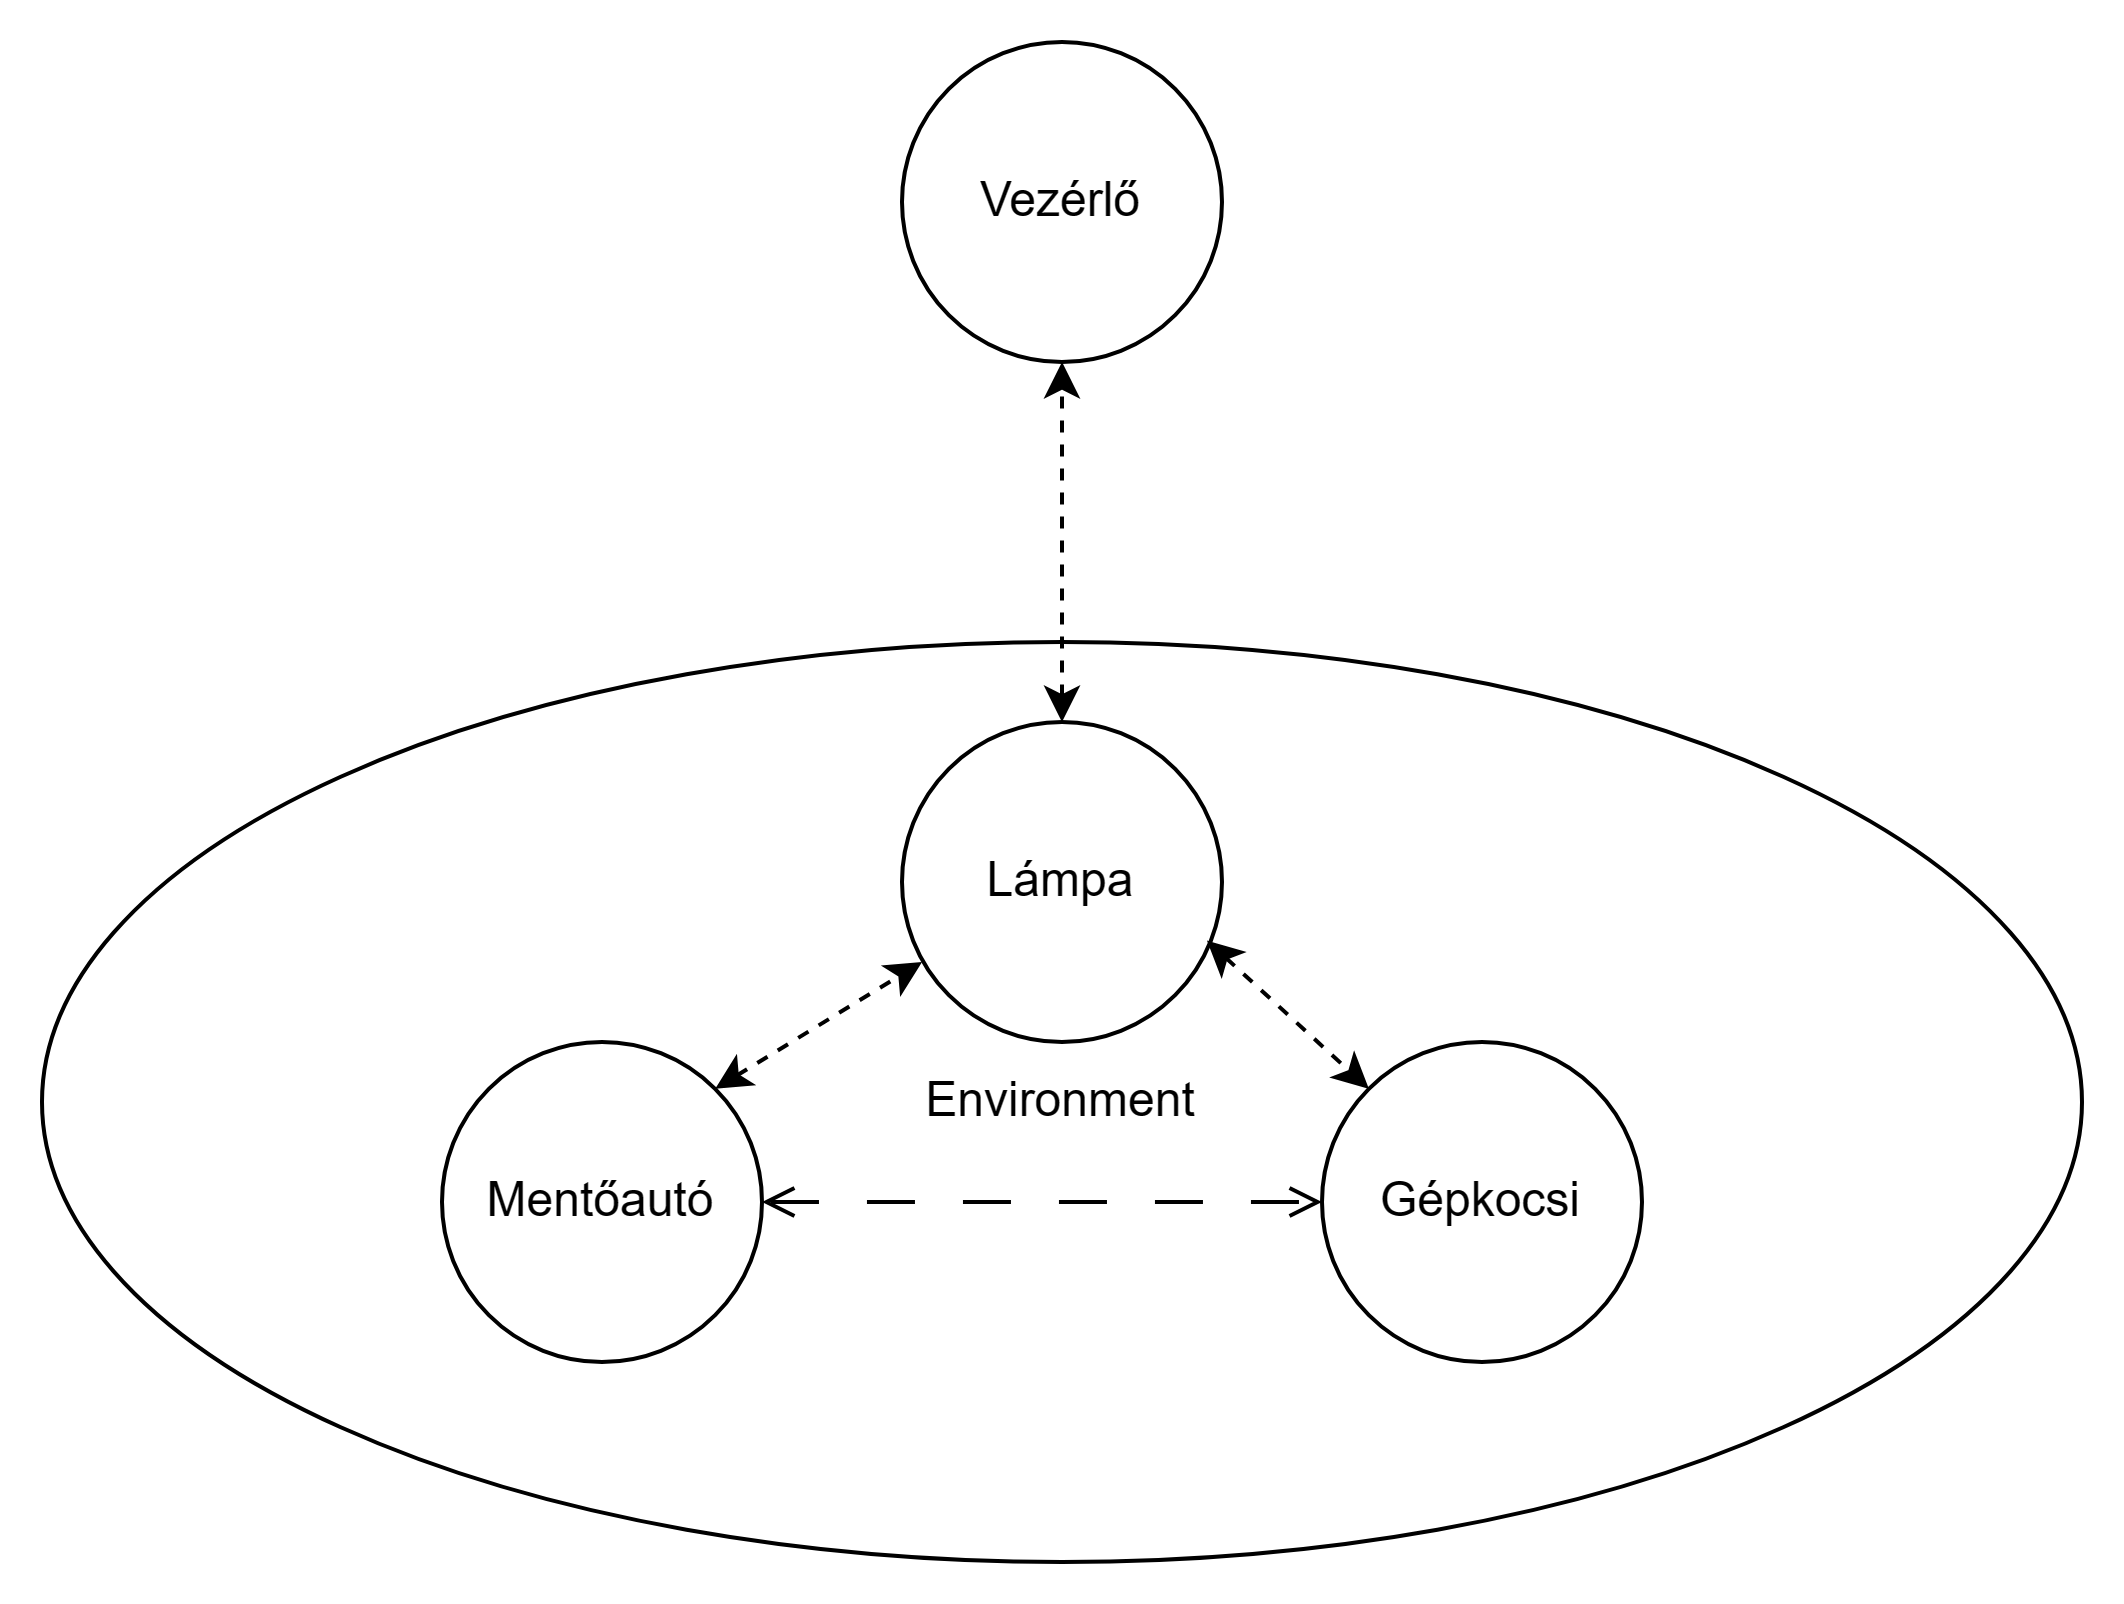
\includegraphics[width=\linewidth, keepaspectratio]{multiagent_diagram.png}
    \caption{A többágenses rendszer ábrája}
\end{figure}

\FloatBarrier

\section{A fejlesztés összefoglalása}
\subsection{Használt környezet}
A fejlesztés során a Jason 3.2.0-ás verzióját használtuk. A projektet a parancssori bináris segítségével
hoztuk létre, majd kigeneráltattuk vele a szükséges gradle fájlokat. Így windows alatt is tudtuk fejleszteni,
tesztelni, futtatni. A program semmilyen egyéb függőséget nem használ.
\subsection{Az ASL felelőssége a programunkban}\label{subsec:asl}
Szinte mindent, ami a BDI szerint az ágensek hatáskörébe tartozik ASL-ben valósítottunk meg. Az ágensek
létrejöttük után kizárólag a környezettel való interakcióra használják a Java kódot, így az érzékelések
rögzítésére, illetve a környezet módosítására.

Hogy ezt megvalósíthassuk, rengeteg szabályt kellett létrehoznunk az ASL-t használva. Bár a modellünk
egy koordináta rendszer, az ágensek az érveléseik során ezt nem tudták volna hatékonyan kezelni.
Ezért az ASL világában a pozíciók az (Oldal, Sáv, Távolság a modell szélétől) hármassal írhatók le.
A szabályok főleg ezekből a pozíciókból következtetnek információkra, mint például melyik sáv kanyarodik
az én oldalamról a céloldalra, melyik lámpa található az én sávom végén, vagy épp melyik sávhoz tartozó
lámpa melyik másik útvonalát blokkolja a kereszteződésben.

Mivel a lámpa ágenseket a mas2j projekt fájlban definiáljuk és hozzuk létre, külön szabály található a
lámpa ágens forrásában, amelyikkel képes azonosítani a saját neve alapján, hogy tulajdonképp melyik sávért
is felel.

Szintén hasznos szabály, amelyik képes meghatározni egy számokat tartalmazó lista összegét. Meglepő, hogy
erre nincs beépített akció a keretrendszerben.

\subsection{A Java felelőssége a programunkban}
Mint ahogyan az \autoref{subsec:asl}-ban említettük, a teljes rendszernek csak azon komponensei találhatók
itt, amit nem lehetett máshogy megoldani. Maga a környezet, amiben léteznek az ágensek, egy ehhez tartozó
modell, a modell nézete és ezeknek egy segédosztálya.

\paragraph{Env.java}
Leszármazik az Environment ősosztályból.
A modell működtetéséért felelős osztály, itt történik az autók és a mentők inicializálása,
a lámpák státuszváltozásainak és a járművek mozgásának nyomonkövetése.
A járművek inicializálása során beállítjuk a kezdeti tudásukat véletlenszerű értékekre, illetve
ellátjuk őket azzal a fontos információval, hogy milyen hosszúak is a sávok.

\paragraph{LogicalCoordinate.java}
Ebben az osztályban váltjuk át a modellbeli Location objektumokat, amely két Integert tartalmaz, x-et és y-t. Így lesznek a koordinátákból side, lane, distance hármasok.
\paragraph{IntersectModelView.java}
A felhasználói interface megjelenítéséért felelős. Az osztály leszármazik a GridWorldView-ból, és annak az initComponents() függvényét felülírva jelenítjük meg a grafikus felhasználói felületet, rajta a 4 darab gombbal, illetve magával a modellel. Ezen osztályban definiáljuk a lámpák rajzolásához szükséges függvényeket is.
\paragraph{IntersectModel.java}
Modell manipulálásáért felelős osztály, amely leszármazik a GridWorldModelből. Konstruktorában történik a modell inicializálása, a falak, illetve lámpák hozzáadása.

\section{A rendszer ismertetése}
\subsection{A felhasználói interfész}
A programnak nincsen futási időben módosítható paramétere, az autók számát, a sávok hosszát illetve a
járművek akciói közt eltelt időt fordítási időben tudjuk beállítani.
A felhasználói felület a jason által beépítetten támogatott GridWorldViewra épül. Mivel a GridWorldModelt
használjuk a modellezésre, a GridWorldView rengeteg alap funkciót automatikusan megvalósít, nekünk csak
a módosítani kívánt megjelenítést kellett felülírnunk.

A felületen található még 4 gomb, amelyekkel a mentőautót tudjuk megjeleníteni a kívánt oldalon. A gombok
bármelyik megnyomása után tiltott állapotba kerülnek, ezzel garantálva, hogy adott időpillanatban
csak egy mentőautó található a modellben. Természetesen amint a születő mentőautó teljesíti feladatát,
elhagyja a világot és megsemmisítésre kerül, a gombok újra aktívvá válnak, készen állva a következő
mentőautó bevetésének megkezdésére.
\subsection{Az ágensprogramok BDI összefoglalása}
\subsubsection{A járművek BDI szempontból}
A járművek abszolút célvezérelt ágensek. Születésük után feltöltésre kerül a kezdeti hiedelem táruk,
(belief base) és egyből ellátjuk őket egy kívánt céllal is. A cél teljesítésése során az autók két szándékkal
rendelkeznek: a sikeres sávváltás, illetve az előre haladás. Ezek ilyen sorrendben élveznek prioritást.
Amint a megfelelő sávba kerül az autó, egyetlen szándék következik a célból, az előrehaladás.

Működésük során a hiedelemtáruk több módon is bővül. A többi autó érzékelése érzék forrású hiedelmekkel
bővíti a tárat. Ha elérik a piros lámpát, saját maguk frissítik be az értékükről alkotott hiedelmüket.
A lámpák állapotáról pedig kommunikáció folytán értesülnek.

\subsubsection{A lámpák BDI szempontból}
A lámpák a járművekkel szemben kizárólag kommunikáció vezérelt ágensek. Nincsen meghatározott céljuk,
szándékuk mindig a járművektől vagy a központtól érkező kommunikáció fogadása és megfelelő feldolgozása.
Éppen ezért az ASL programjában nem is található teljesítménycél létrehozása, illetve arra való terv sem.

A lámpa kezdeti hiedelemtárja csak a saját sávjának azonosítására szolgál. Ezután a sávba érkező autók
értékével telik meg sorra.

Több terv található a kommunikációra épülve. A lámpa tudja fogadni az járművektől azt az információt, hogy
sikeresen beléptek a kereszteződésbe, ekkor törli a saját hiedelemtárjából az adott jármű értékét.

Ezen kívül reagál a központ által érkező összes utasításra, amik alapján zöldre vagy pirosra váltja magát.
Illetve kérés esetén válaszol az összegyűlt autók értékével.

\subsubsection{A központ BDI szempontból}
A központ kezdeti hiedelemtára szintén csak szabályokkal van tele, amiket fel tud használni a különböző
kalkulációk során. A központ ezután két cél között váltogat: a kereszteződés teljes megállítása, illetve
aukció kihírdetése a zöldre váltáshoz. Miután a központ bekérte az összes lámpa licitjét, felállít egy sorrendet
köztük. Ezután végigmegy a győztestől a vesztes felé. Minden lámpát, aki adott be érvényes licitet, és
a lámpa által feloldott útja nem keresztezi az aktuális aukcióban már engedélyezett lámpák útját, engedélyez,
és az adott lámpa útjait felveszi a listába, a további ellenőrzés érdekében.

Tehát a központ célja minél több lámpa zöldre váltása, és ennek érdekében szándéka minden lámpát megvizsgálni,
és lehetőség szerint engedélyezni. Tiltó állapotban pedig célja az összes lámpa letiltása, és az egyetlen érvényes
szándéka ezt valósítja meg.
\subsection{A MAS összefoglalása}


\end{document}